\documentclass[12pt]{ucthesis}

\usepackage{etex}
\usepackage[morefloats=125]{morefloats}
\usepackage[hyphens]{url}
\usepackage{subfig}
\usepackage{graphicx}
\usepackage{tabularx}
\usepackage{amssymb}
\usepackage{amsmath}
\usepackage[letterpaper]{geometry}
\usepackage[overload]{textcase}
\usepackage{color}
\usepackage[nonumberlist,toc]{glossaries}
\usepackage{wrapfig}
\usepackage{longtable}
\usepackage{morefloats}
\usepackage{float}
\usepackage{listings}
\usepackage{makecell}
\usepackage{appendix}
\usepackage{cleveref}
\usepackage[]{algorithm2e}
\usepackage{titlesec}
\usepackage[breaklinks=true,hidelinks,pdfusetitle]{hyperref}
\usepackage{ifthen}
\usepackage{pgfplots}

\makeindex
\makeglossaries

% Shrink the size of headers
\titleformat{\chapter}[display]
        {\normalfont\normalsize\centering}
        {\ifthenelse{\equal{\thechapter}{A}}{APPENDICES\\[4.3ex]}{}\chaptertitlename\ \thechapter}
        {0pt}{\normalsize\uppercase}
\titlespacing*{\chapter}{0pt}{-20pt}{4.3ex plus .2ex}


\titleformat*{\section}{\normalsize\bfseries}
\titleformat*{\subsection}{\small\bfseries}
\titleformat*{\subsubsection}{\small\bfseries}
\titleformat*{\paragraph}{\small\bfseries}
\titleformat*{\subparagraph}{\small\bfseries}

\bibliographystyle{abbrv}

\setlength{\parindent}{0.25in} \setlength{\parskip}{6pt}
\geometry{verbose,nohead,tmargin=1in,bmargin=1in,lmargin=1.5in,rmargin=1in}
\setcounter{tocdepth}{2}

% Different font in captions (single-spaced, bold) ------------
\newcommand{\captionfonts}{\small\bf\ssp}

\newcommand{\mycaption}[2]{\caption[#1 --- #2]{#1 --- #2}}

\makeatletter  % Allow the use of @ in command names
\long\def\@makecaption#1#2{%
  \vskip\abovecaptionskip
  \sbox\@tempboxa{{\captionfonts #1: #2}}%
  \ifdim \wd\@tempboxa >\hsize
    {\captionfonts #1: #2\par}
  \else
    \hbox to\hsize{\hfil\box\@tempboxa\hfil}%
  \fi
  \vskip\belowcaptionskip}
\makeatother   % Cancel the effect of \makeatletter
% ---------------------------------------

% Define Appendix refs
\crefname{app}{appendix}{appendices}
\Crefname{app}{Appendix}{Appendices}

\begin{document}

% Declarations for Front Matter
\title{Highly scaleable open-world game simulation}
\author{Ian Dunn}
\degreemonth{December} \degreeyear{2016} \degree{Master of Science}
\defensemonth{December} \defenseyear{2016}
\numberofmembers{3}
   \chair{Professor Zoe Wood, Ph.D. \linebreak Department of Computer Science}
   \othermemberA{---, Ph.D. \linebreak Department of Computer Science}
   \othermemberB{---, Ph.D. \linebreak Department of Computer Science}
\field{Computer Science} \campus{San Luis Obispo}
\copyrightyears{seven}


\maketitle

\begin{frontmatter}

% Custom made for Cal Poly (by Mark Barry, modified by Andrew Tsui).
\copyrightpage

% Custom made for Cal Poly (by Andrew Tsui).
\committeemembershippage

\begin{abstract}
Open-world video games give players a large environment to explore along with increased freedom to navigate and manipulate that environment.
These requirements pose several problems that must be addressed by the game’s graphics engine.
Often there are a large number of visible objects as well as objects comprised of large amounts of geometry, such as terrain.
An open-world graphics engine must be able to render large environments at varying levels of detail and smoothly transition between detail levels to provide a believable experience.
It is also necessary to employ special techniques to both store and generate the geometry for the environment.

In this thesis we present a system for generating and rendering large exterior environments, with a focus on terrain, vegetation, and structures.
We utilise a feature-based procedural generation algorithm to create environments with some artistic control.
This algorithm produces content that can be rendered at multiple levels of detail.
The terrain is rendered volumetrically to support caves, overhangs, and cliffs, but is also rendered using heightmaps to allow for large view distances.
Vegetation is implemented using procedurally generated meshes and impostors.
The generation itself is accomplished by using a hierarchical feature representation to piece together noise samples.
The terrain is editable in real time, which limits our ability to pre-generate or cache large amounts of geometry, and also limits the number of assumptions we can make with regard to visibility.

We support a view distance of at least 25 miles in each direction, though distance objects are rendered only if very large, and at low resolution.
The heightmap terrain used to achieve this view distance consists of over 360,000 triangles.
Our target frame rate is 60fps on a gaming desktop computer and 30fps on a gaming laptop computer.

\end{abstract}

\begin{acknowledgements}
\noindent
Thanks to:
\begin{itemize}
    \item Andrew Guenther, for uploading this template
\end{itemize}

\end{acknowledgements}

\tableofcontents

\listoftables

\listoffigures

% Add CHAPTER into table of contents.
\addtocontents{toc}{%
   \noindent CHAPTER
}

\end{frontmatter}

\pagestyle{plain}

\renewcommand{\baselinestretch}{1.66}



\chapter{Introduction}

Many of the top selling video games of all time are ``open-world'' games.
{\em Minecraft}, {\em Grand Theft Auto V}, and {\em The Elder Scrolls V: Skyrim} are all good examples.
One of their defining characteristics is that they offer players an expansive world to play and explore in.
Those three titles alone have a combined total of over 190 million copies sold, and

Creating such a world is not a simple task, however.
It is not straightforward to write a game engine that can render rolling hills, towering mountains, and dense forests.
Nor is it simple to create these exterior environments, either through the careful work of artists or the expensive application of procedural generation techniques.


\section{A World Of Geometry}

The primary source of difficulty in this field is the tremendous scale.
Landscape scenes require incredible amounts of geometry to represent everything from the terrain itself to the trees and water.
It is not be possible to store the entirety of the visible scene in a modern computer's memory.

Game developers attempting to render an open-world game must use techniques that not only load in different parts of the environment as they are needed, but also load those parts at differing detail levels.


\section{Our System}

This paper describes a game engine designed to render large exterior environments.
We discuss related work from a variety of topics, and present a system which incorporates many of these ideas.
Our system procedurally generates and renders terrain, vegetation, water, and atmospheric effects.

For terrain generation, we implement a system for picking between a variety of landscape generators using noise algorithms.
This system determines not only the elevation and color of the terrain, but also parameters such as forestation and material properties.

The generated terrain is rendered using a novel voxel implementation for nearby terrain and a heightmap-based implementation for distant terrain.
The distant terrain system supports a view distance of 25 miles in all directions.

Forests are rendered by the system using a combination of three different rendering approaches.
Terrain, forests, and other scene elements including the sky and water render at 170 frames per second with a 2560x1440 resolution.
See Figure~\ref{fig:system1} for an overview of the system.

\begin{figure}
  \centering
    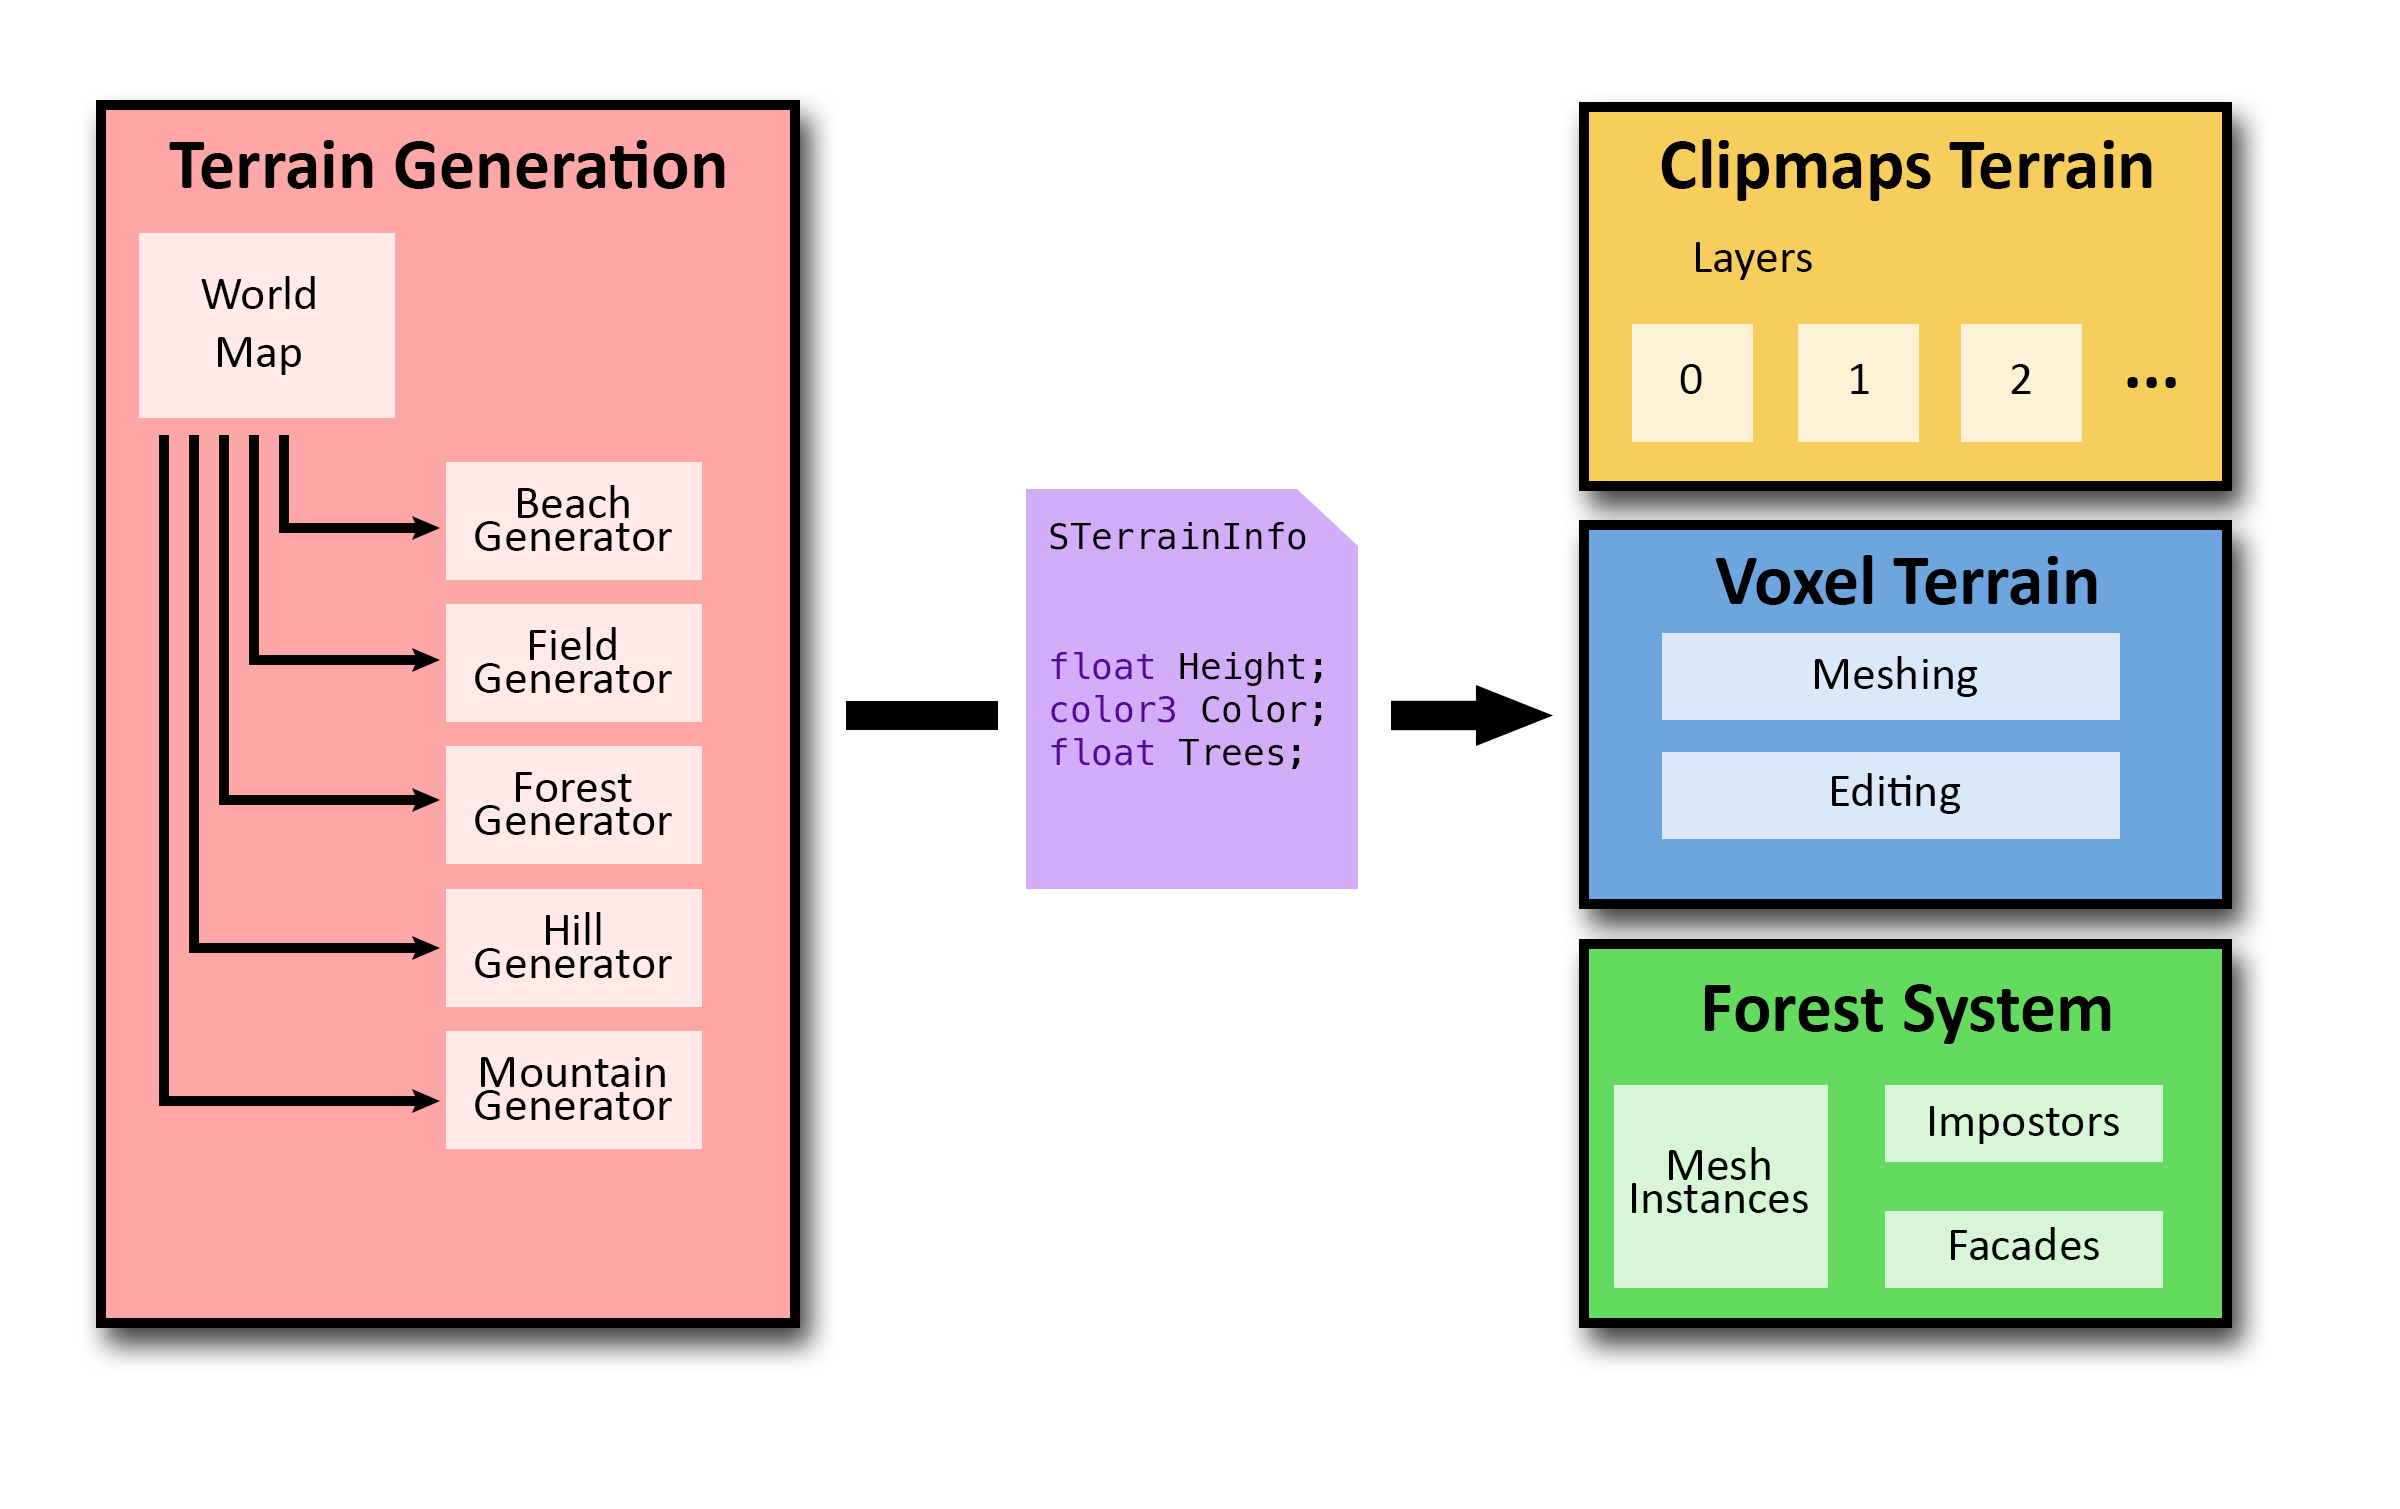
\includegraphics[width=1.0\textwidth]{figures/SystemDiagram.png}
  \caption{Overview of the presented system}
  \label{fig:system1}
\end{figure}


\chapter{Background}

\editor{Need references and citations in this chapter}

\section{Computer Graphics}

Computer Graphics is the process of using computers to produces images.
In real-time applications, this involves using a GPU to rasterize triangles and other primitives.
This process involves producing the geometry to be rendered and then performing a lighting calculation that determines the color of each pixel in the resulting image.

\section{Level of Detail}

\section{Terrain Rendering}

Terrain rendering is a particular subset of computer graphics that is concerned with producing images of terrain.
Terrain is important because it plays a large role in the appearance of outdoor scenes, but it is difficult to render because it requires a tremendous amount of geometry.
Terrain rendering methods usually focus on employing level-of-detail algorithms that make it possible to render close-up terrain in high detail and far-away terrain in low detail.
\editor{Need to define `detail' and reference an image}
Some of the main challenges these techniques aim to solve are creating the visual transitions between two areas that are rendered at different detail levels, and implementing a scheme to load in new data smoothly when the viewpoint changes.

\section{Terrain Generation}

There are many possible sources of terrain data.
Acquired data from the real world is often available.
The USGS provides satellite data for much of the world's surface.
Some game engines also use terrain editing tools that allow artists to sculpt terrain manually.

However, it is also possible to implement algorithms that procedurally construct terrain.
The advantage of using procedurally generated terrain is that it requires less time/effort intensive than artistically creating a terrain, and it does not require much or any disk space (as opposed to using acquired data which can be very large).

Procedural terrain generation methodologies usually employ one or more of the follow techniques.

\begin{itemize}
\item Physical process simulations
\item Fractal processes
\item Noise algorithms
\end{itemize}

\subsection{Physical process simulations}

Real terrain is shaped by erosion, the gradual shaping of landscape caused by water, wind, and other forces.
Some terrain generation techniques simulate these physical processes on a starter dataset to create realistic surfaces. \cite{hydrology}

\subsection{Fractal processes}

Another technique for generating terrain is a fractal process, some algorithm that operates on geometry to add detail and which can be re-applied at smaller and smaller scale until a highly detailed surface results.
The most common form of fractal process is the Diamond-square Algorithm which sequentially subdivides and modulates a regular grid.

\subsection{Noise Algorithms}

Noise algorithms are similar to fractal processes but more heavily based in mathematics.
The most typical way that noise algorithms are used is by generating a patch or formula for noise (typically in 2 dimensions, though sometimes more) and employing a technique called fractional Brownian motion to create a heightmap.
Noise is generally a signal that varies randomly.
Coherent noise is a special brand of noise that is more useful for generation purposes.
As a random signal, it is reasonable to expect that a large change in domain results in a random change in output for a given noise function.
Coherent noise has the property that for small changes in domain, only a small change in output will result.

\subsubsection{Coherent Noise}

There are two major types of coherent noise.

% \subsubsection{Value noise}

The most simple is value noise.
Value noise is generated by calculating random numbers at fixed intervals and interpolating between the values.

% Value noise works by using a pseudo-random number generator to generate a set of initial random values, then interpolate between those values.

% \subsubsection{Gradient noise}

Another type of coherent noise is gradient noise.
Gradient noise is generated by calculating vectors at a fixed interval, then performing a dot product to calculate intermediary values instead of interpolating.
It is a numerically similar process to value noise, but produces noise with more variance - that is, more detail in higher frequencies.

% Gradient noise is a modification of value noise where gradient vectors are calculated at grid points, and noise is generated by calculating the dot product between a gradient vector and the offset to the calculated location.
% The purpose of this technique is the improve the mathematical properties of the

\subsubsection{Fractional Brownian Motion}

Fractional Brownian motion is a technique for taking a noise function and adding detail at higher frequencies.
The general approach is:
\begin{enumerate}
\item Take a noise function as input
\item Double the frequency and halve the amplitude of the noise function, then add it to itself. This is called the second octave.
\item Double again the frequency and halve again the amplitude of the noise function, then add this too into the sum. This is the third octave.
\item Repeat Step 3 for subsequent octaves until amplitude is close enough to zero that added octaves produce no change in the output, or until desired amount of detail is reached.
\end{enumerate}

In general you do not need to exactly double the frequency or halve the amplitude each octave, but can fine tune these values e.g. by multiplying the frequency by 1.2 and the amplitude by 0.3.

\subsubsection{Ridged Multifractal}

An additional step can be added before summing each individual octave.
By first taking the negated absolute value of each generated noise value, a ridged version of fractional brownian motion can be created.
This technique is commonly referred to as Ridged multifractal, or RMf.

\subsubsection{Noise Distortion}

Ridged multifractal works on fractal brownian motion by modifying the range of each noise function, but it is also possible to modify the domain in a similar fashion.
Using two additional FBM generators, an offset vector can be produced for each sample of the height generator.
This technique helps break up the homogeneous appearance of generated terrain by shrinking and expanding different areas.


\section{Voxels}


\section{Screen-space Ambient Occlusion}

\subsection{Ambient Occlusion}

\subsection{Screen-space}

\subsection{HBAO+}



\chapter{Related Works}

\section{Publications}

\subsection{Geometry Clipmaps: Terrain Rendering Using Nested Regular Grids}

Geometry clipmaps is a good example of a highly scaleable system. The cost of doubling visible terrain area is low, making it trivial to expand the side of visible geometry beyond the practical limitations of floating point numbers. \cite{geometry_clipmaps}

This is a terrain rendering technique.
The general approach is to center a regular grid of vertices around the viewpoint, then nest this grid in a larger grid of vertices, and so forth.
Each nested grid has double the resolution of the outer grid such that there is increased detail closer to the viewer.
A torroidally updating texture heightmap is used at each level so that new data can be loaded incrementally.

\subsection{Terrain Generation Using Procedural Models Based on Hydrology}

This is a terrain generation technique, though the authors also touch on their approach to rendering the terrain surface.
One interesting aspect to note is their novel approach to storing the terrain which focuses on a hierarchy of features instead of only considering geometry.
I think this technique could prove a useful inspiration for designing other scaleable systems besides terrain.

The main point of this paper is to generate terrain using a physically accurate hydrology model.
The results speak for themselves - using their technique produces visually stunning images.

\subsection{Terrain Synthesis from Digital Elevation Models}

This paper is mostly interesting because of the quality of the resulting terrains.
Their technique involves sampling real terrain data using a user-controlled shape/template to generate a new terrain.

For some games this process has tremendous potential for allowing some artist control of the surface while still importing tremendous detail that doesn't need to be artistically controlled.
For my system, it may be worth exploring how the resulting terrain appears when the user-controlled texture is itself procedurally generated.

\subsection{Socially competent AI characters}

Some interesting work in the area of creating authentic characters with realistic motivations. \cite{socially_competent}

\section{Commercial Video Games}

\subsection{Skyrim}

Skyrim has two artificial intelligence systems under the name ``Radiant'' which are of some interest. The first, Radiant AI, is a system for establishing character personalities by assigning them tasks to perform on a daily basis. Characters also maintain a relationship with the player which affects their reactions to player actions. For example, characters who are friendly to the
player may invite the player to dinner if they barge into the character's house in the late evening, whereas characters which are not friendly may be upset by this occurrence.

On the surface these systems seem promising but their implementations are heavily scripted and reliant on pre-existing planning and forethought. There are also a considerable number of character quirks which have given Skyrim a reputation for humorously dumb AI. \cite{skyrim_gamespy} \cite{skyrim_ign} \cite{gameinformer_skyrimtech} \cite{skyrim_nesmith_radiant} \cite{skyrim_whatsnew}

\subsection{Minecraft}

At first glance, Minecraft appears to be an open world game because of the significant amount of freedom afforded to players both in game choices and even in style of gameplay.

Many players of Minecraft tout the impressive scale of the game because the worlds which are procedurally generated are theoretically quite expansive. However, deeper analysis shows that the scale of Minecraft is actually quite limited. While the world size in terms of raw horizontal distance is quite impressive, this massive size is only possible through a severely limited vertical scale in which the highest mountains rise only 60 meters above sea-level, and the deepest oceans are only another 60 meters below the surface.

In general, the horizontal scale around the player is also quite limited. Without any sophisticated level-of-detail system, view distance is severely low
and only allows players to see objects that are fairly nearby. Coupled with the previously discussed vertical limitations, the world (from a player's perspective) is actually quite small.

In terms of implementation, Minecraft simply ignores scale as defined in this paper's introduction. There is only a single level of abstraction employed by
the simulation engine - events which are nearby occur, and anything which is beyond that ``nearby'' threshold is cached out and entirely static until it is
revisited. This is entirely unsatisfactory from a world-simulation standpoint, and disqualifies Minecraft as an open-world game.


\chapter{Generation} \label{generation}

\begin{figure}
	\centering
		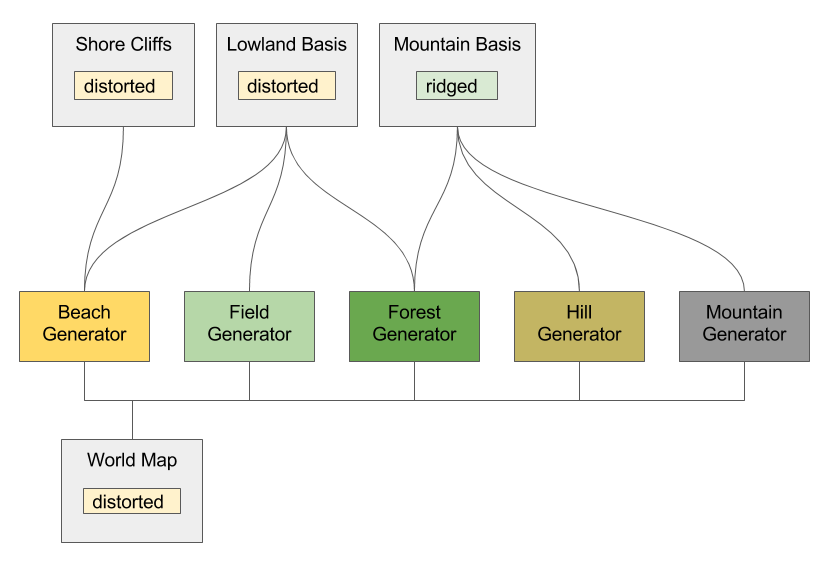
\includegraphics[width=1.0\textwidth]{figures/generation_flowchart.png}
	\caption{Terrain generation system overview, showing the type of noise generators used.}
	\label{fig:gen_overview}
\end{figure}

Our terrain generation algorithm creates a world with large continents that contain beaches, forests, hills, and mountains.
The algorithm uses a low-frequency world map to determine continent outlines and region boundaries.
For finely sampled terrain values, the values of the world map are used to select and influence custom generators for each region type.
See Figures \ref{fig:gen_overview} and \ref{fig:worldmap}.
The world map is discussed in Section \ref{sec:worldmap} and the different region generators are discussed in \ref{sec:region}

\begin{figure}
	\centering
		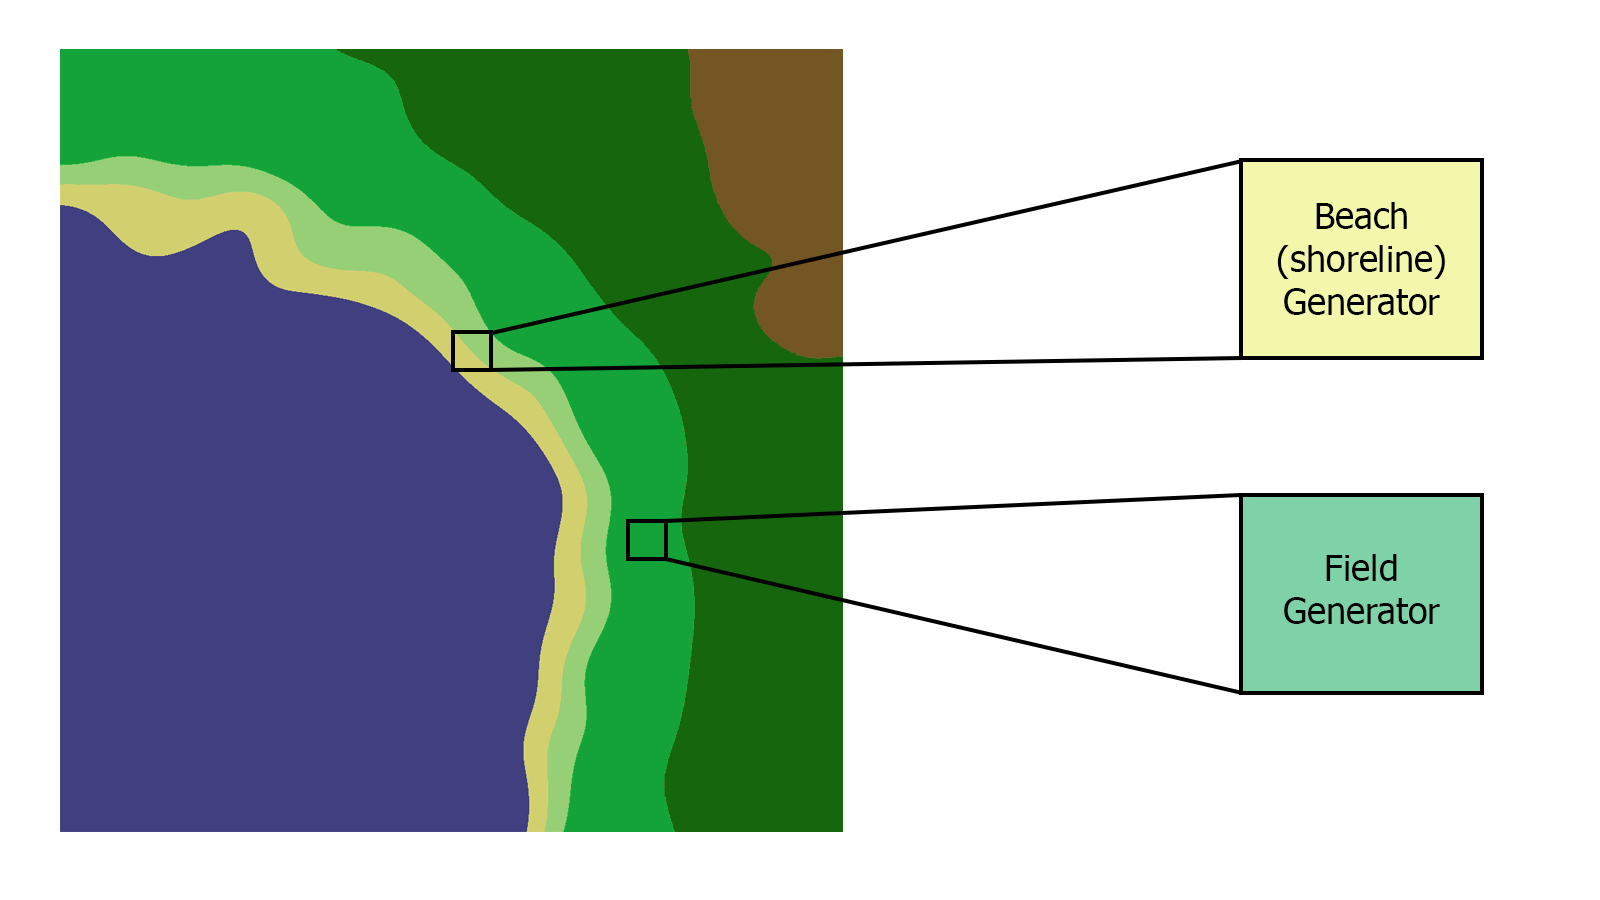
\includegraphics[width=1.0\textwidth]{figures/worldmap.png}
	\caption{Example world map section and generator selection.}
	\label{fig:worldmap}
\end{figure}

\section{World Map} \label{sec:worldmap}

The terrain is generated by first establishing a low-frequency world map, then selecting from a series of different landscape generators based on general elevation.
The world map uses a single distorted fractal noise layer with a box ramp to force oceans at all borders.

A low number of octaves is used (four, in our implementation) to guarantee a lack of high-frequency details.
This makes it useful for generating features without having areas that swap between multiple region types unrealistically.
Figure \ref{fig:worldmap} shows an example of the smooth isolines generated by the world map.

\section{Regions} \label{sec:region}

For rendering, the terrain values need to be generated at 1 foot postings.
We also need color values to shade the ground, and a forestation value to determine how to place trees.

Values from the world map are used to pick a particular set of terrain generation rules, referred to as a region.
The return value from the world map generator has a theoretical range from -1 to 1, but most values tend to be between -0.7 and 0.7.
This range is divided into regions with low values mapping to low elevation regions and high values mapping to high elevation regions.
See \ref{tab:regions} for the exact world map values used to determine regions.

\begin{table}
	\centering
	\begin{tabular}{ || c | c | c || }
		\hline
		Region & Minimum & Maximum \\ [0.5ex]
		\hline\hline
		Ocean & -1 & 0 \\
		\hline
		Shore & 0 & 0.05 \\
		\hline
		Field & 0.05 & 0.15 \\
		\hline
		Forest & 0.15 & 0.30 \\
		\hline
		Hills & 0.30 & 0.45 \\
		\hline
		Mountain & 0.45 & 1.0 \\ [1ex]
		\hline
	\end{tabular}
	\caption{Region boundaries from the world map values.}
	\label{tab:regions}
\end{table}

The world map can usually be used to generate color values, i.e. the color from the image in \ref{fig:worldmap} is used by each region generator.
However, the Mountains generator in Section \ref{sec:mountains} does some additional coloring.

For each region, a ``region delta'' is calculated to indicate how far into a region the engine is currently generating data for.
A region delta of \(0.0\) indicates the boundary with the next lower elevation region, \(1.0\) indicates the higher boundary, and \(0.5\) indicates the middle of the region.

The region types used by the engine are: Oceans, Beaches, Fields, Forests, Hills, and Mountains.

While each region generator is individually responsible for generating elevation values, some noise sources are shared between the different regions so that smooth transitions can be generated.
As an example, the Oceans, Fields, and Forests generators all share a distorted fractal noise source.

\subsection{Oceans and Fields}

The oceans, fields, and forests generators all simply add some high-frequency noise to the world map value with some scaling.
This generates small sandy hills below water for Oceans, small grassy hills for Fields, and tree-covered hills for Forests.

\subsection{Beaches}

Beaches serve as a transition between oceans and fields.
Beaches may contain a cliff partway between the shoreline and the transition to the field region.

This cliff is generated by applying a vertical offset to any baseline value above a certain threshold.
The offset is applied gradually over a small area so that the cliffs are not completely abrupt, but have a horizontal dimension of a few feet.
As the baseline elevation approaches the transition to Fields, the offset is tapered off to give cliffs some additional prominence.
See Figure~\ref{fig:beach_cliffs}.

The cliff generation offset function is as follows, where v is the map value:

$$
shoreline(v) = \left\{\begin{array}{lr}
	0, & \text{for } 0 \leq x \leq \text{cliff\_start} \\
	\text{cliff\textunderscore size} * \text{cliff\_falloff} * \text{cliff\_gain}, & \text{for } \text{cliff\_start} < x \leq 1
\end{array}\right\}
$$

Where cliff\_gain and cliff\_falloff are both computed as follows, but clamped from 0 to 1:

$$
\text{cliff\_gain} = \frac{v - \text{cliff\_start}}{\text{cliff\_range}}
$$

$$
\text{cliff\_falloff} = \frac{x - (\text{cliff\_start} + \text{cliff\_range})}{\text{falloff\_range}}
$$

The exact size, shape, and shoreline distance of the cliffs are configured by the parameters cliff\_start, cliff\_range, cliff\_size, and falloff\_range.
Relic uses additional noise layers to add variance to these parameters, and adds applies a gain function to both cliff\_gain and cliff\_falloff to create a smoother final appearance.

\begin{figure}
	\centering
		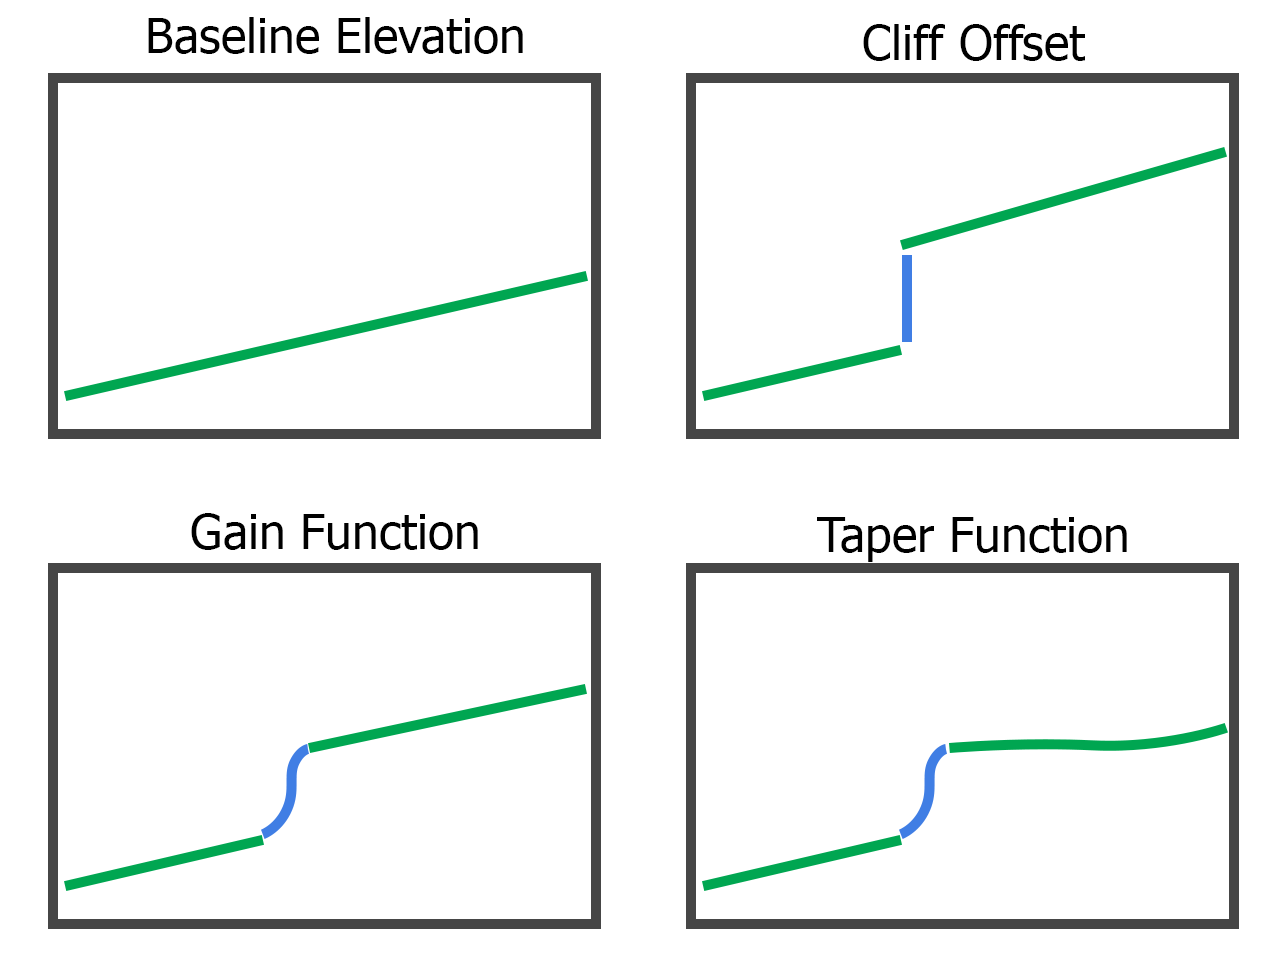
\includegraphics[width=0.8\textwidth]{figures/beachcliffs4x4}
	\caption{Beach cliff generation}
	\label{fig:beach_cliffs}
\end{figure}

\subsection{Forests, Hills, and Mountains} \label{sec:mountains}

The Forests, Hills, and Mountains regions both use a custom version of a ridged fractal generator.

For the first two octaves of noise, a standard gradient noise sample is used instead of the ridged version.
This helps reduce the sharpness of some peaks and hides some unnatural artifacts that sometimes occur.
Figure \ref{fig:original_ridged} shows the first few octaves of a ridged fractal generator without this modifications.
The ridge lines established by the second octave have a large effect on the resulting image even as more octaves are added.
The smoothness of these lines creates circular artifacts in the resulting terrain.
Figure \ref{fig:my_ridged} shows the first few octaves of a ridged fractal generator with this modification.
The effect is similar to lowering the amplitude and increasing the frequency of a normal ridged fractal generator but with large-scale variation preserved.

\begin{figure}
	\centering
		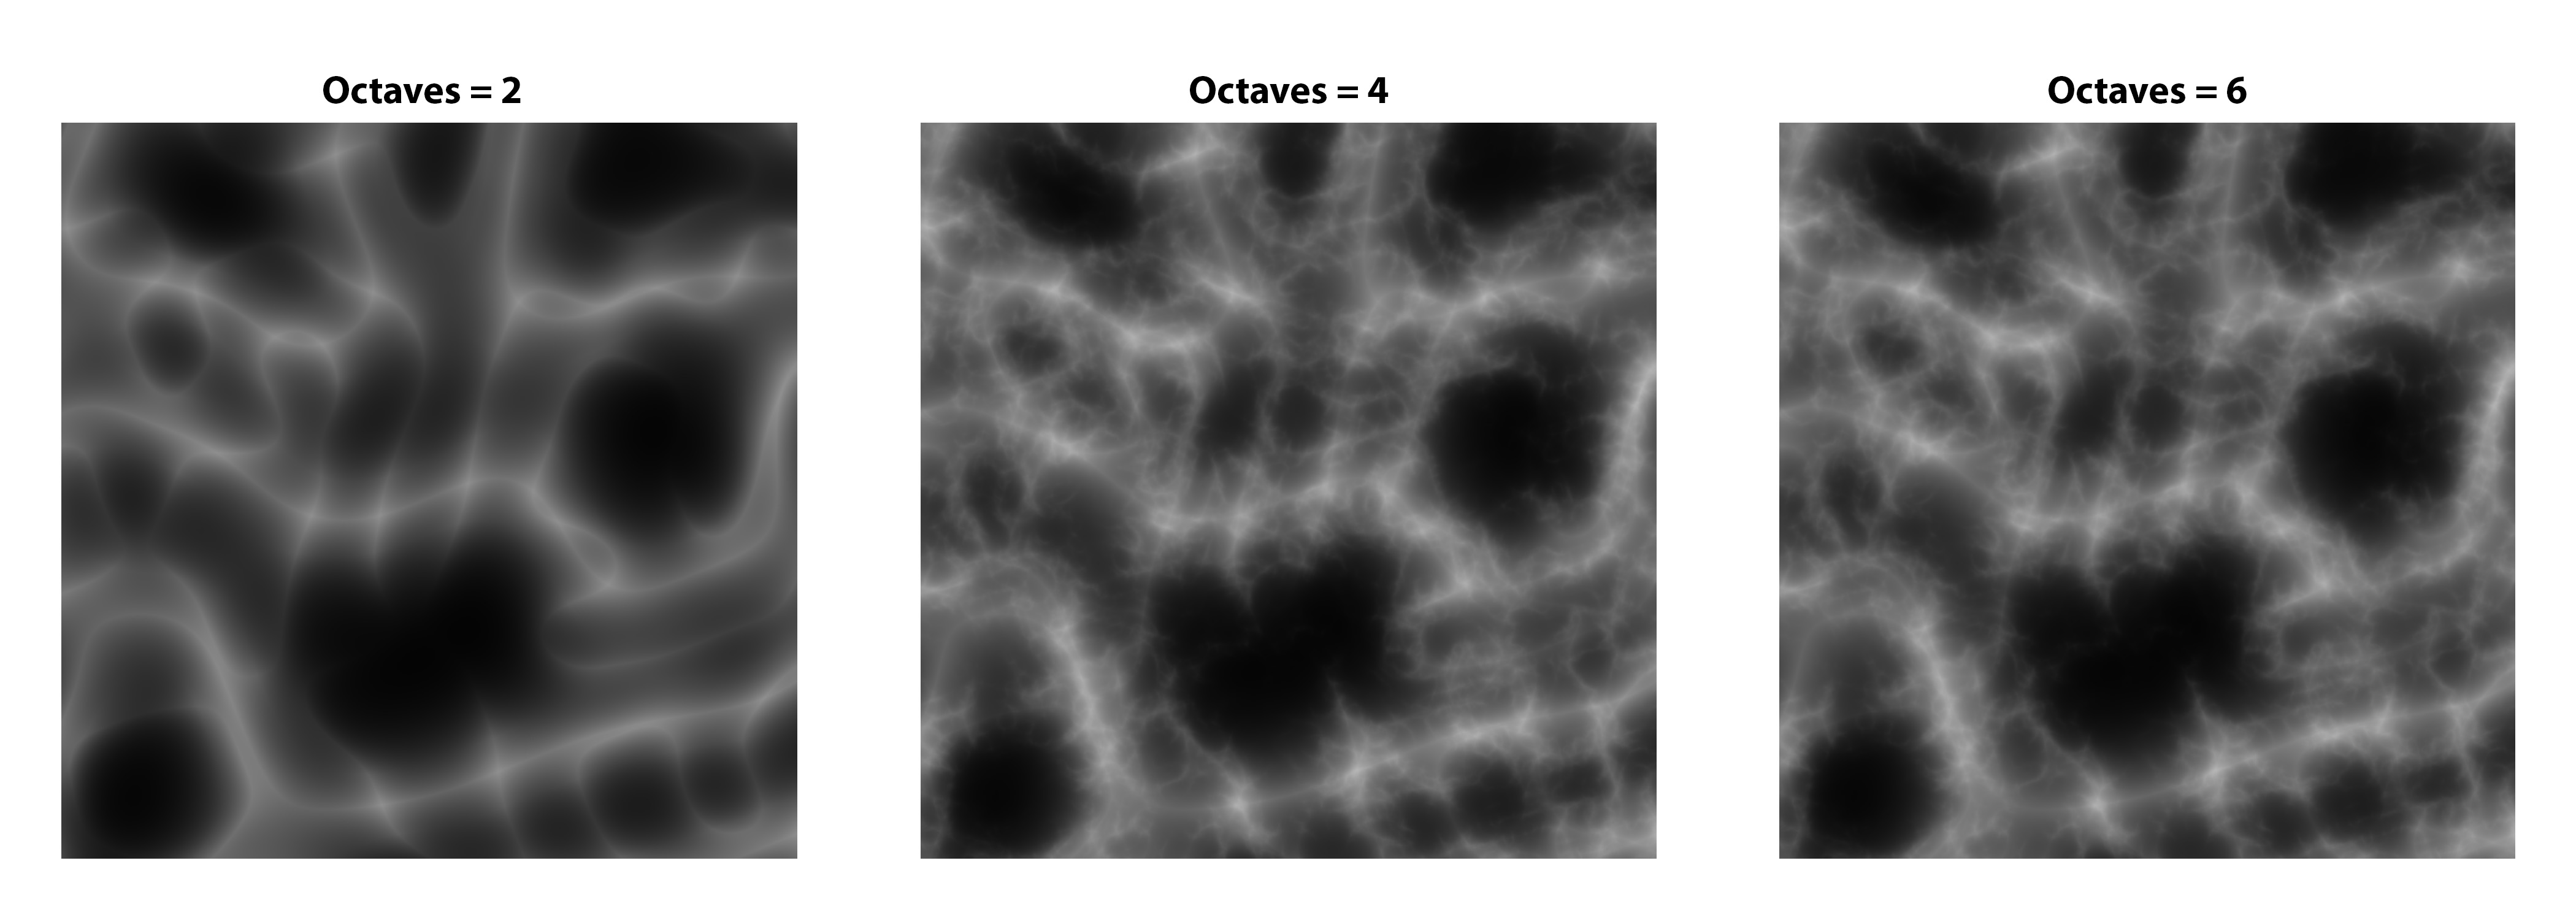
\includegraphics[width=1.0\textwidth]{figures/original_ridged}
	\caption{Two, Four, and Six octaves of a ridged fractal generator without our modification of using a standard fractal noise source for the first two octaves.}
	\label{fig:original_ridged}
\end{figure}

\begin{figure}
	\centering
		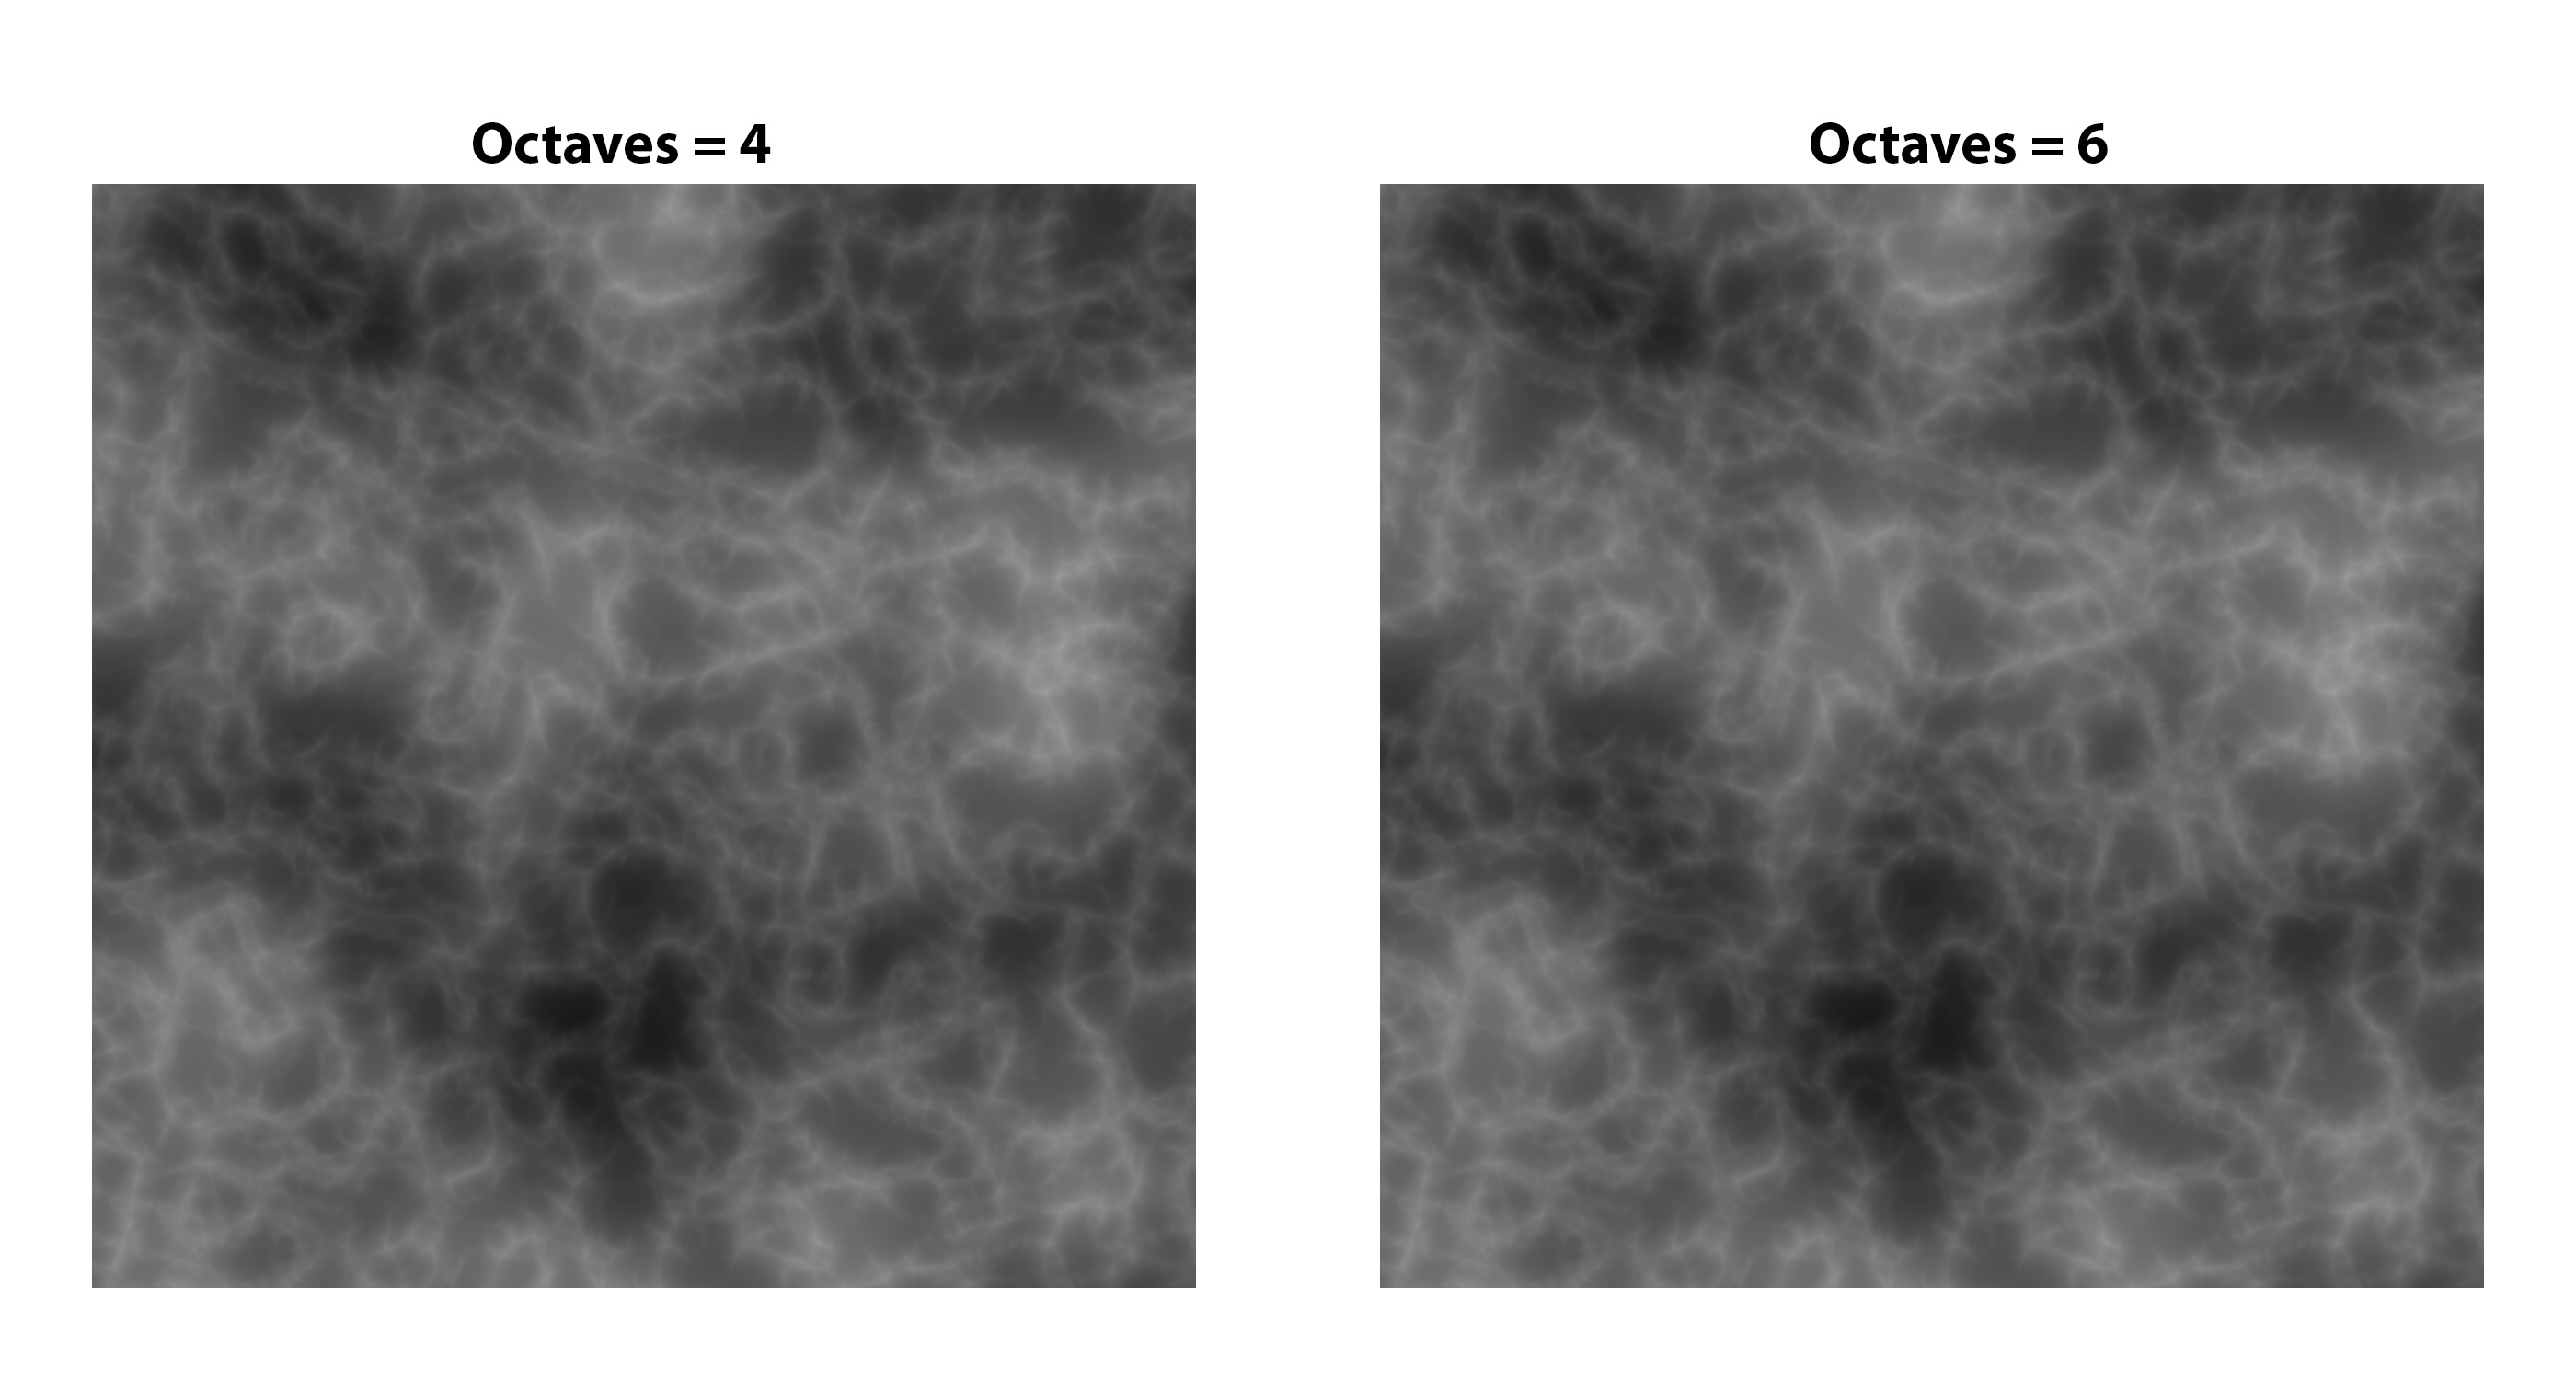
\includegraphics[width=1.0\textwidth]{figures/my_ridged}
	\caption{Four and Six octaves of the ridged fractal generator used by Relic, where a standard fractal noise source is used for the first two octaves.}
	\label{fig:my_ridged}
\end{figure}

In addition, a hilliness parameter is added to help smoothly transition between mountains and hills.
When hilliness is 0, the standard absolute value is used.
At hilliness of 1, the input value is squared instead to produce a parabolic shape.
Hilliness values between 0 and 1 interpolate between these two shapes.

At the low edge of Hill regions, a hilliness value of 1 is used along with low overall amplitude.
These same parameters are used at the high edge of the Forest region, and create smooth rolling hills of medium height.
In the Mountain region, hilliness falls to 0 and amplitude increases to create sharp ridge lines and towering peaks.

Mountain regions are colored by adding snow coverage over the region color specified by the world map.
Snow is added whenever the angle between the normal of the surface and the up vector is smaller than some value.
For high elevations, a large angle is used, and at low elevations a small angle is used.

\section{System Overview}

The use of a world map generator defines at a large scale what type of geometry to generator, including continent outlines and region boundaries.
Values generated by the world map are used to pick a particular region generator and transition smoothly between each region.
The regions, in order of elevation, are Oceans, Beaches, Fields, Forests, Hills, and Mountains.
Oceans and Fields have simple geometry - just some low amplitude noise to create small hills and variations.
Beaches serve as a ramp between Ocean and Field regions, with a cliff generated partway up the shore.
Forests, Hills, and Mountains use a custom ridged fractal generator to create ridged mountaintops and rolling hills.


\chapter{Rendering}

\begin{figure}
  \centering
    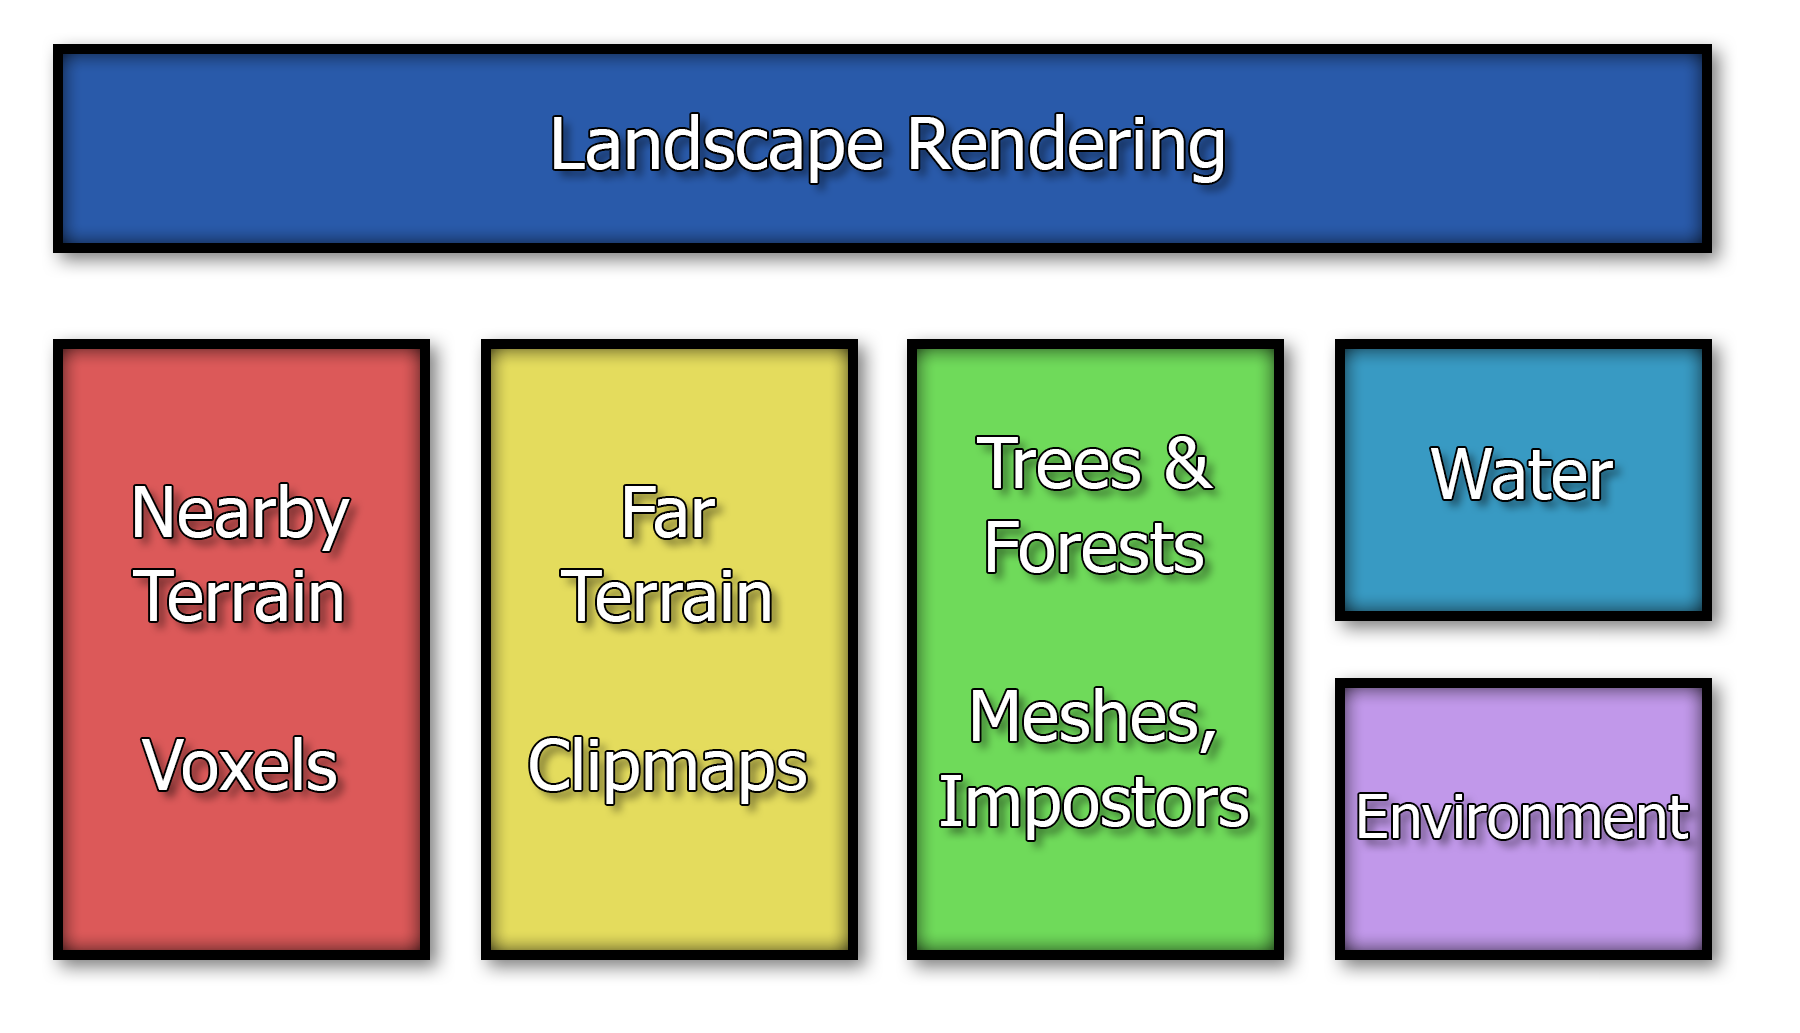
\includegraphics[width=0.8\textwidth]{figures/RenderSystem}
  \caption{Landscape rendering system overview}
  \label{fig:renderoverview}
\end{figure}


Our landscape rendering system consists of three primary components - a nearby terrain renderer, a distant terrain renderer, and a forest renderer.
The nearby terrain renderer uses a meshing algorithm influenced by voxel terrain systems (Section \ref{voxterrain}).
This mesh generation is expensive but is necessary for meaningful player interaction and is limited to a very narrow region around the viewpoint.
Far terrain is rendered using a modified implementation of geometry clipmaps (Section \ref{clipterrain}).
The nature of the clipmaps algorithm makes it possible to extend the terrain view distance substantially with minimal overhead.
Our forest system uses mesh instances, impostors, and a similar representation called facades to render vast forests (Section \ref{forests}).
The system is designed to render a large number of individual trees with the highest performance possible.
In addition to these three primary components, our system also renders water and other additional environment aspects, discussed in Sections \ref{sec:water} and \ref{sec:env}.
See Figure \ref{fig:renderoverview} for an overview of the system.

\section{Nearby Terrain} \label{voxterrain} %%%%%%%%%%%%%%%%%%%%%%%%%%%%%%%%%%%%%%%%%%%%%%%%%%%%%%%%%%%%%%%%%%%%%%%%%%%%%%%%%%%%%%%%%%%%%%%%%%%%%%%%%%%%%%%%%%%%%%%%%%%%%%%%%%%%%%

Nearby terrain is rendering using a pseudo-voxel representation designed to allow for sloped surfaces while maintaining intuitive live editing capabilities.
A voxel algorithm that uses uniform voxel size is simple to implement and manage but is poorly suited to represent sloped surfaces.
Fully volumetric terrain implementations allow for arbitrary slopes but are less intuitive for manipulation by players and navigation by AI.
We utilize a pseudo-voxel system that allows for diagonal faces in addition to solid voxels.
This system allows for simple grid-based editing and simple physics calculations, while allowing sloped polygonal faces that are more aesthetically pleasing than simple voxels.

\subsection{Voxel algorithm}

In principle, the system works by breaking down each individual voxel into 8 sub-voxels (one for each corner of the cube) and generating diagonal faces based on which of these sub-voxels are occupied.
However, certain sub-voxel configurations are considered degenerate and are automatically trimmed to a lesser configuration.
For example, in our system any pseudo-voxel with only a single sub-voxel occupied is automatically trimmed to an empty voxel.
In this case the trimming occurs because there is no diagonal face to represent just a single corner of a voxel.
Figure \ref{fig:minimumvoxel} shows the pseudo-voxel with the fewest possible sub-voxels, four.

\begin{figure}
	\centering
		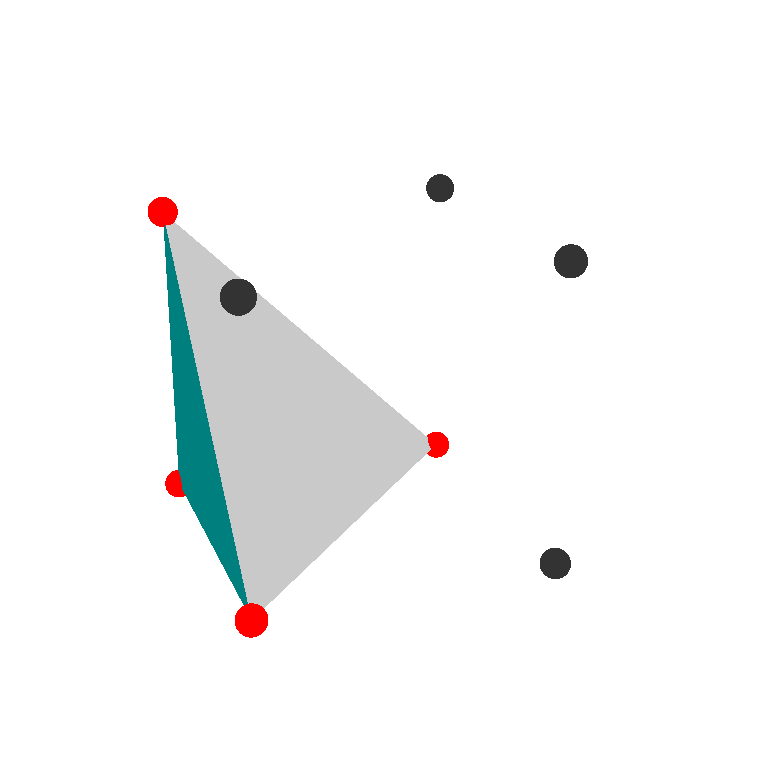
\includegraphics[width=0.5\textwidth]{figures/minimumvoxel.png}
	\caption{Red spheres indicate a full sub-voxel, grey indicates an empty sub-voxel.}
	\label{fig:minimumvoxel}
\end{figure}

The system can therefore trivially trim any pseudo-voxel configuration with fewer than four sub-voxels.

The system also trims certain pseudo-voxel configurations to a simpler configuration.
See Figure \ref{fig:voxelrejected} for an example.

\begin{figure}
	\centering
		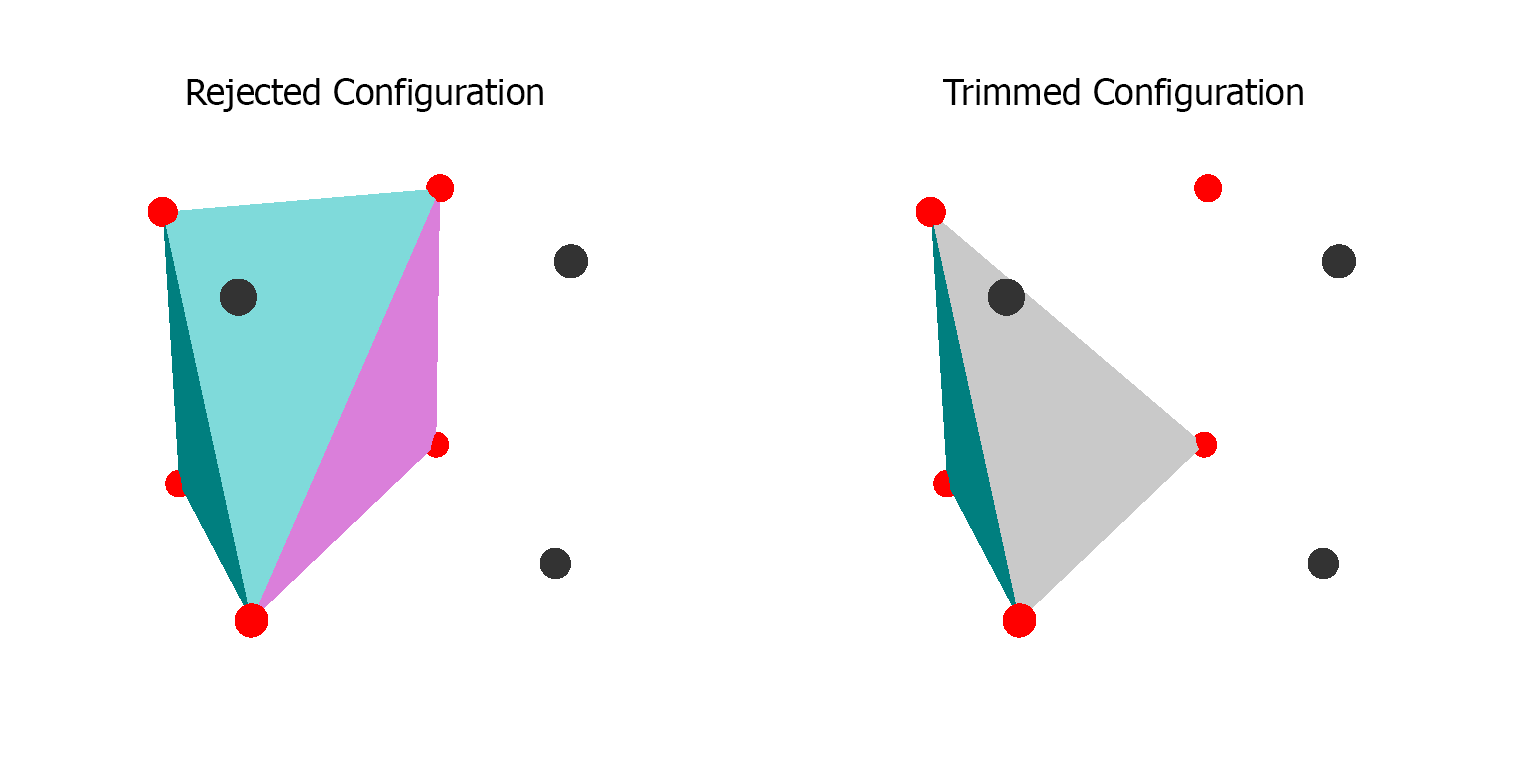
\includegraphics[width=1.0\textwidth]{figures/voxelrejected.png}
	\caption{
		Red spheres indicate a full sub-voxel, grey indicates an empty sub-voxel.
		The image on the left shows a possible triangulation for this sub-voxel configuration.
		However, our algorithm rejects this configuration and instead generates the triangulation on the right.
	}
	\label{fig:voxelrejected}
\end{figure}

This trimming is performed to make the voxel triangulation easier to understand at a glance, and also to preserve smooth slopes of generated terrain.
See Figures \ref{fig:trimcomparison1} and \ref{fig:trimcomparison2} for a comparison between untrimmed and trimmed sub-voxel configurations.

\begin{figure}
	\centering
		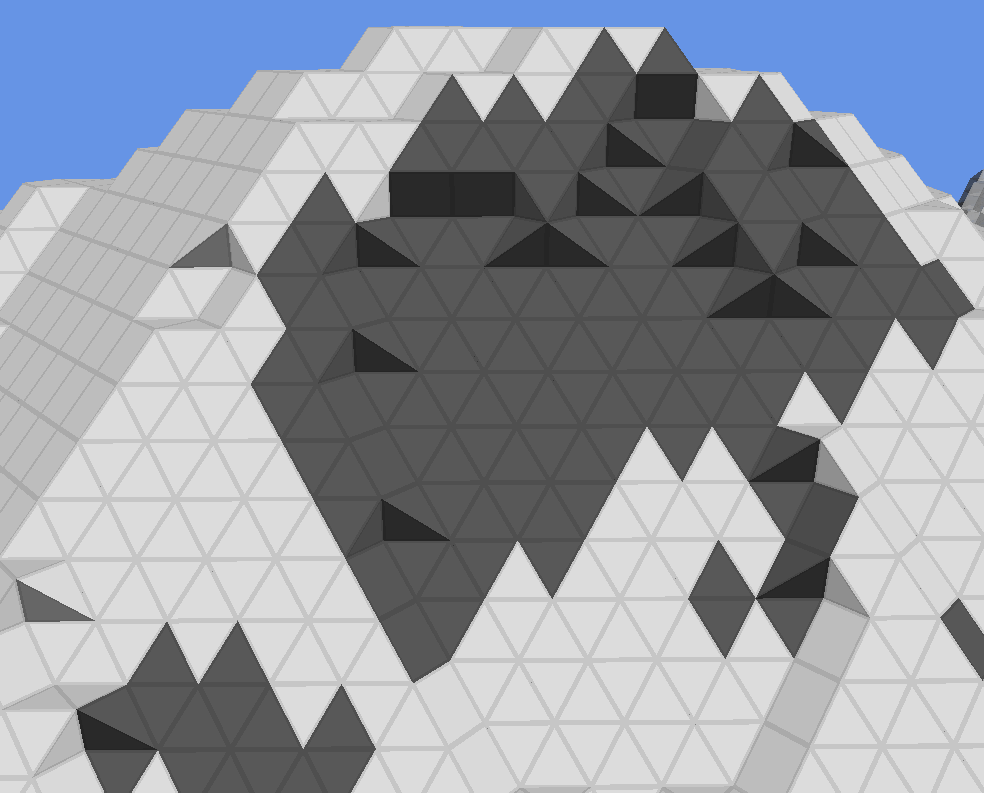
\includegraphics[width=0.75\textwidth]{figures/trimcomparison1.png}
	\caption{
		Voxel triangulation of a mountaintop without sub-voxel trimming enabled.
	}
	\label{fig:trimcomparison1}
\end{figure}

\begin{figure}
	\centering
		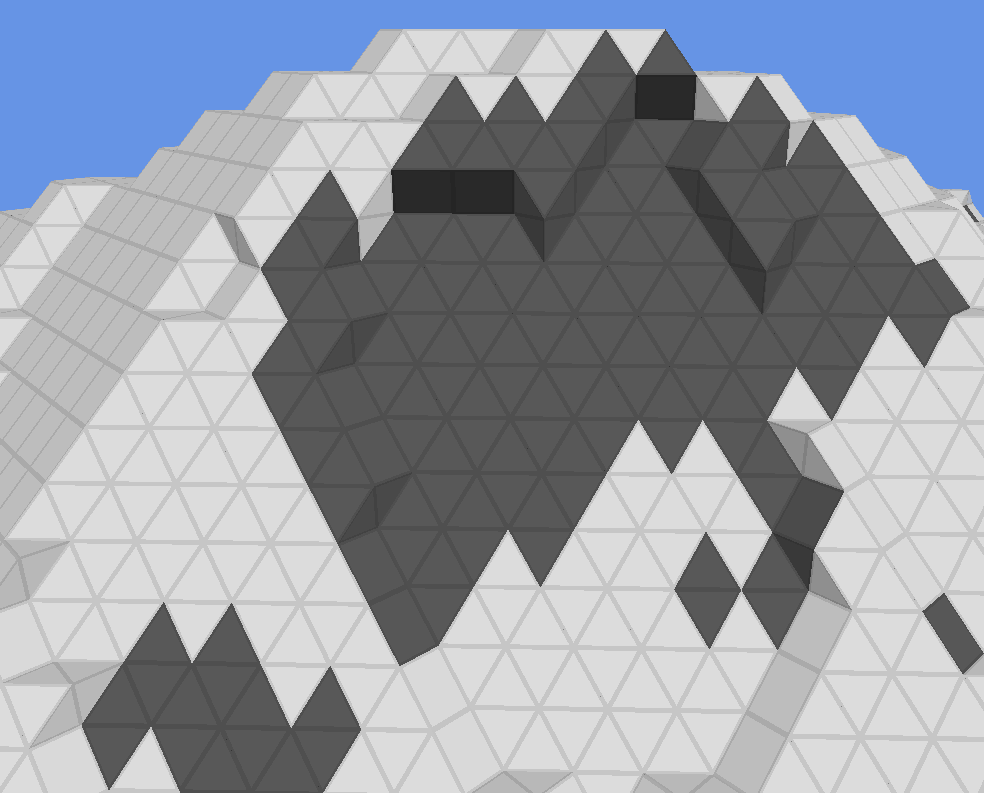
\includegraphics[width=0.75\textwidth]{figures/trimcomparison2.png}
	\caption{
		Voxel triangulation of a mountaintop with sub-voxel trimming enabled.
	}
	\label{fig:trimcomparison2}
\end{figure}

\subsection{Face Generation}

Triangles are generated for each pseudo-voxel configuration using lookup tables for efficiency and simplicity.
Triangles are divided into two categories: interior and exterior.

\subsubsection{Exterior Faces}

Exterior triangles are the triangles that would normally be generated by a simple voxel system - the faces of a cube.
Exterior triangles are checked against each neighboring pseudo-voxel for visibility.
In the trivial case, a completely solid voxel surrounded entirely by solid voxels produces no triangles, since all exterior triangles are occluded by the exterior faces of each neighboring voxel.

\subsubsection{Interior faces}

Interior faces are what make the pseudo-voxel system interesting - any diagonal face that caps a partial pseudo-voxel.
See Figure \ref{fig:interiorfaces2} for a table of all interior faces.

\begin{figure}
	\centering
		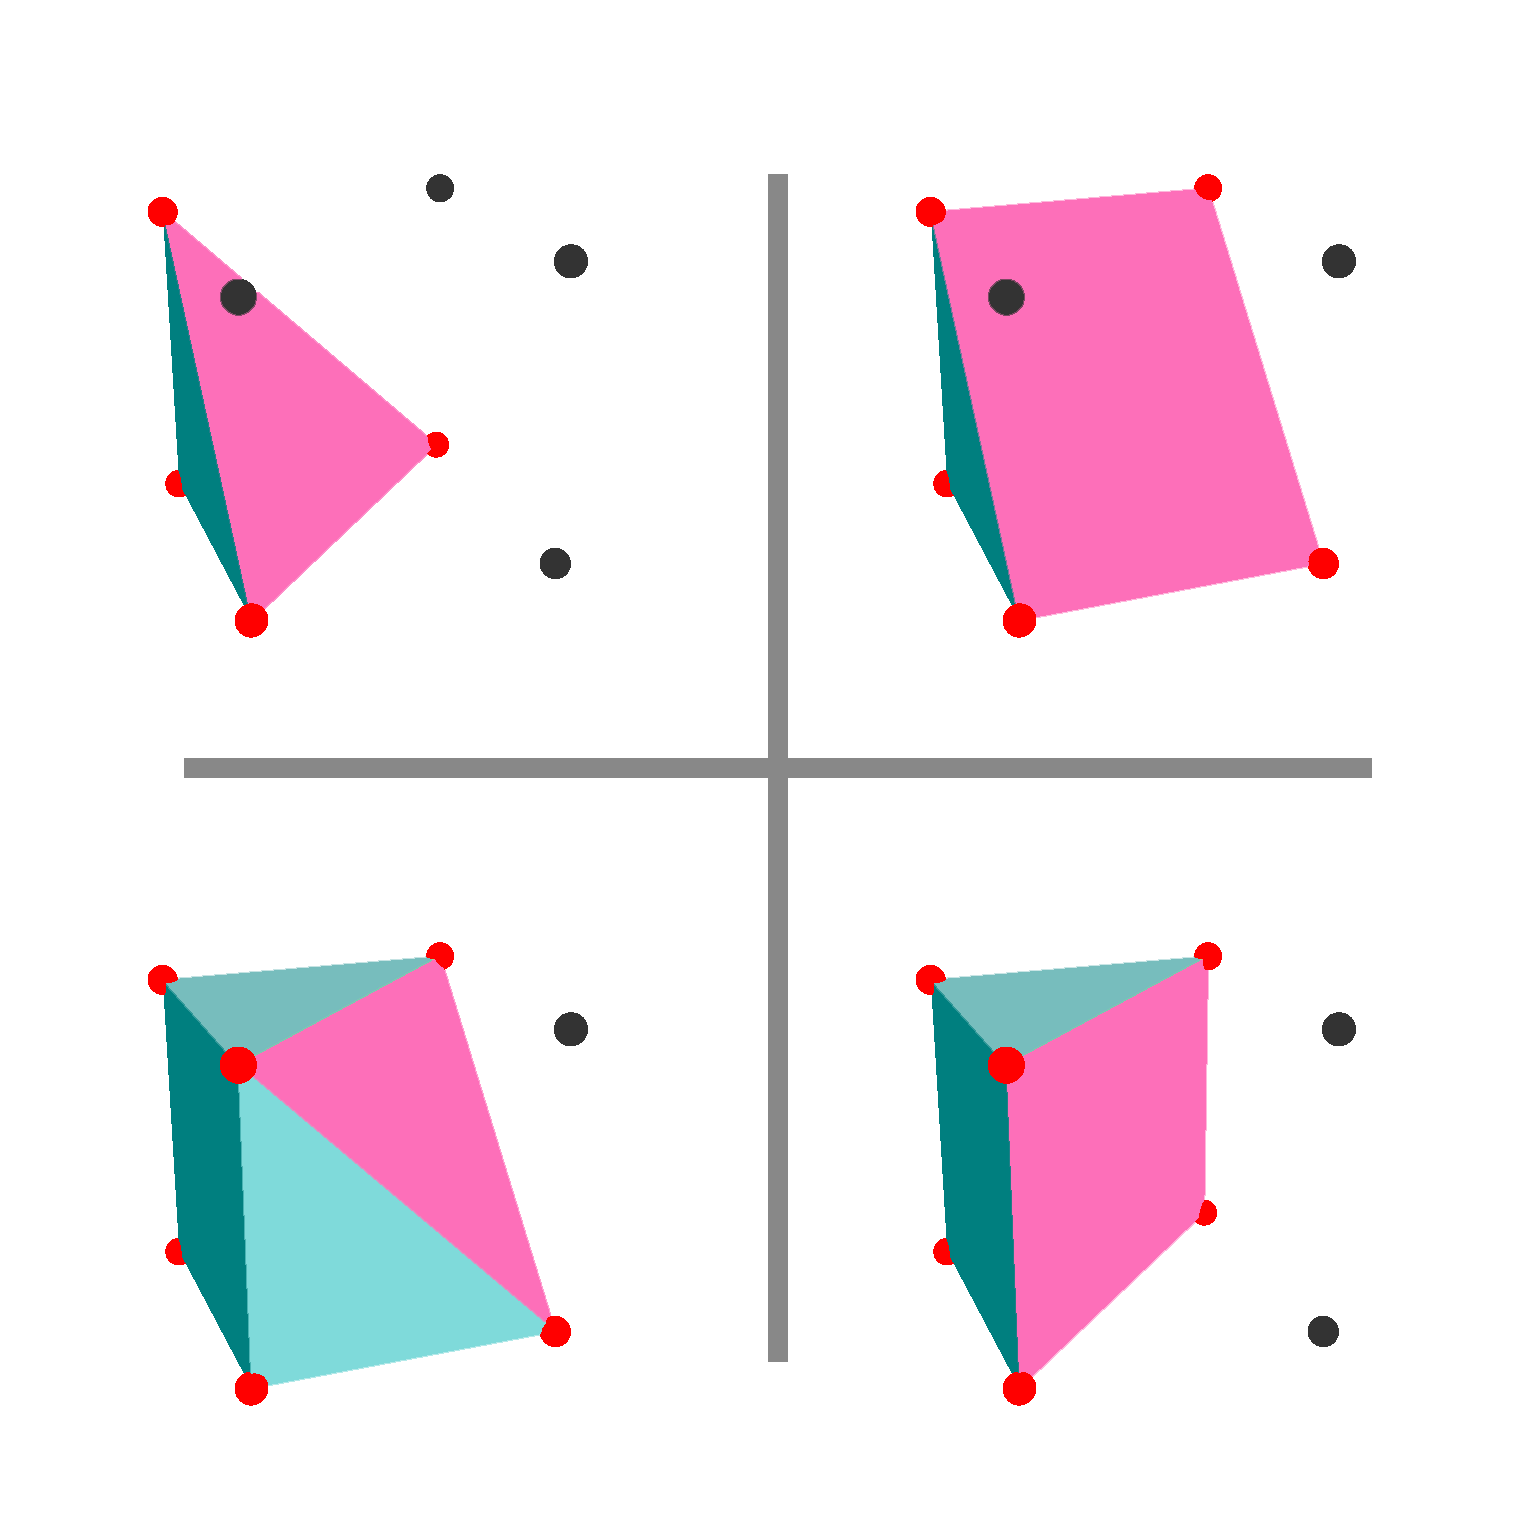
\includegraphics[width=0.75\textwidth]{figures/interiorfaces2.png}
	\caption{
		Example of the four types of interior face.
		Each pink face is an interior face.
		Note that this is just one possible orientation of each class of interior face, but each class can be oriented in either four or eight directions.
		(The left two classes have eight orientations and the right two have four).
	}
	\label{fig:interiorfaces2}
\end{figure}

\subsection{Rendering}

The world is divided into cube chunks for which a triangle mesh is generated.
Each chunk tracks its neighbors in all six face directions so that occluded exterior faces can always be accurately detected.
This means that a ring of non-visible chunks must be loaded around all visible chunks, since no visible chunk can have an unloaded neighbor.

Screen-space ambient occlusion is used to help visual understanding of the voxel terrain shape.


\section{Far Terrain} \label{clipterrain} %%%%%%%%%%%%%%%%%%%%%%%%%%%%%%%%%%%%%%%%%%%%%%%%%%%%%%%%%%%%%%%%%%%%%%%%%%%%%%%%%%%%%%%%%%%%%%%%%%%%%%%%%%%%%%%%%%%%%%%%%%%%%%%%%%%%%%%%%%%%%%%%%%%%%%%%%%%%%

Far terrain is rendered using a flat-shaded implementation of geometry clipmaps with a few modifications.

\subsection{Pre-calculated Index Buffer}

The original geometry clipmaps implementation recalculates index buffers pre-frame so that each layer can grow and expand organically.
This makes it possible to seamlessly transition to lower-resolution terrain when the viewpoint moves rapidly.

However, our system locks the size of each layer so that the index buffers can be pre-calculated.
This was found to significantly reduce CPU overhead

\subsection{Normal Calculation}

Since our terrain is flat-shaded for a polygonal effect, the per-quad normals provided by a normal map must be inaccurately applied to two triangles.
We also found that normal calculation from our procedural generation system incurred significant CPU overhead.
Accurate normal calculation in transition regions was also difficult.

Our implementation uses a per-triangle normal calculation in a geometry shader so that accurate normals are always calculated for each triangle.
This saves significant CPU time as normals don't need to be pre-calculated or sent to the GPU normal map.
The addition of the geometry shader was found to not have a significant decrease in rendering performance.


\section{Forests} \label{forests} %%%%%%%%%%%%%%%%%%%%%%%%%%%%%%%%%%%%%%%%%%%%%%%%%%%%%%%%%%%%%%%%%%%%%%%%%%%%%%%%%%%%%%%%%%%%%%%%%%%%%%%%%%%%%%%%%%%%%%%%%%%%%%%%%%%%%%%%%%%%%%%%%%%%%%%%%%%%%%

Our vegetation system currently supports rendering a large number of low-poly spruce trees, but could be expanded to support other types of vegetation.
The system uses three levels of detail: mesh instances, impostors, and mesh facades.

Trees are rendered in groups similar to the chunk system used by nearby terrain.
Mesh instances and impostors render many trees per group, whereas the mesh facade renders a single mesh to represent each group.

\subsection{Mesh Instances}

The mesh instances layer simply uses instance rendering to draw the tree model in several places.

\subsection{Impostors}

The impostors layer draws a billboard for each tree in the group.
During initialization, the colors and normals of the tree model are rendered to textures for use in drawing each impostor.
The impostors are locked in their X and Z axis rotation so that the base of the impostor always rests on the ground, and to reduce artifacts when the camera is high above or below the impostor.
See Figure \editor{need comparison of a tree billboard rotating around all axis}.
The rotation around the Y-axis is used to rotate the normals of the impostor so that lighting is accurate for impostors in all directions.

\subsection{Mesh Facades}

The final layer uses a simple mesh to represent a group of trees.
The appearance of this mesh is quite simplistic but at large view distances it is sufficient to represent a group of trees.
See Figure \editor{need close-up and distant view of a facade}.

\section{Water} \label{sec:water} %%%%%%%%%%%%%%%%%%%%%%%%%%%%%%%%%%%%%%%%%%%%%%%%%%%%%%%%%%%%%%%%%%%%%%%%%%%%%%%%%%%%%%%%%%%%%%%%%%%%%%%%%%%%%%%%%%%%%%%%%%%%%%%%%%%%%%%%%%%%%%%%%%%%%%%%%%%%%%%%%%%


Our water system uses the geometry of our far terrain (geometry clipmaps) implementation for simplicity.

Instead of offsetting each vertex by a heightmap value, however, we used summed Gerstner waves in the vertex shader.
This provides both a vertical offset and a normal to use for rendering.

The result is expensive, but simple and looks reasonable.


\section{Environment} \label{sec:env} %%%%%%%%%%%%%%%%%%%%%%%%%%%%%%%%%%%%%%%%%%%%%%%%%%%%%%%%%%%%%%%%%%%%%%%%%%%%%%%%%%%%%%%%%%%%%%%%%%%%%%%%%%%%%%%%%%%%%%%%%%%%%%%%%%%%%%%%%%%%%%%%%%%%%%%%%%%%%

The system renders a billboard to represent the sun and a sky sphere with vertex colors to represent the sky.

Lighting for all other objects in the scene uses three directional lights: one for direct sunlight, one for scene reflection of sunlight, and one for sky light.
The sunlight has high bright white color and points from the sun position towards the scene.
The scene reflection light has dim white color and points in the opposite direction of the sunlight, with the Y component clamped to zero.
The sky light points directly downward (negative Y) and has soft blue color.

Our system also implements a simple atmospheric scattering simulation by applying fog to each rendered fragment based on scene depth.
The fog color interpolates between dark blue for near fragments and the sky color for far fragments.


\iffalse \bibliography{../bibliography.bib} \fi

\chapter{Results}


\section{Voxels}

The size of voxel chunks affects rendering performance and the cost of modification.
Since modifying the terrain requires the entire chunk mesh to be reconstructed, it is ideal to have smaller chunks.
However, larger chunk sizes reduce the number of draw calls.

\editor{Graph of rendering performance for different chunk sizes}

\editor{Graph of modification cost i.e. digging for different chunk sizes}

\section{Clipmaps}

One motivation for using geometry clipmaps is an even distribution of screen space to polygon.
\editor{need figure of polygonal screen-space density compared to a simple grid}

Another advantage of geometry clipmaps is the exponential relationship between layer count and view distance.
Figure \ref{fig:clipmaps_plot_1} shows the relationship between clipmap layers, view distance, and frame time in milliseconds for a scene containing only the clipmaps terrain and a skybox.

\begin{figure}
	\centering
		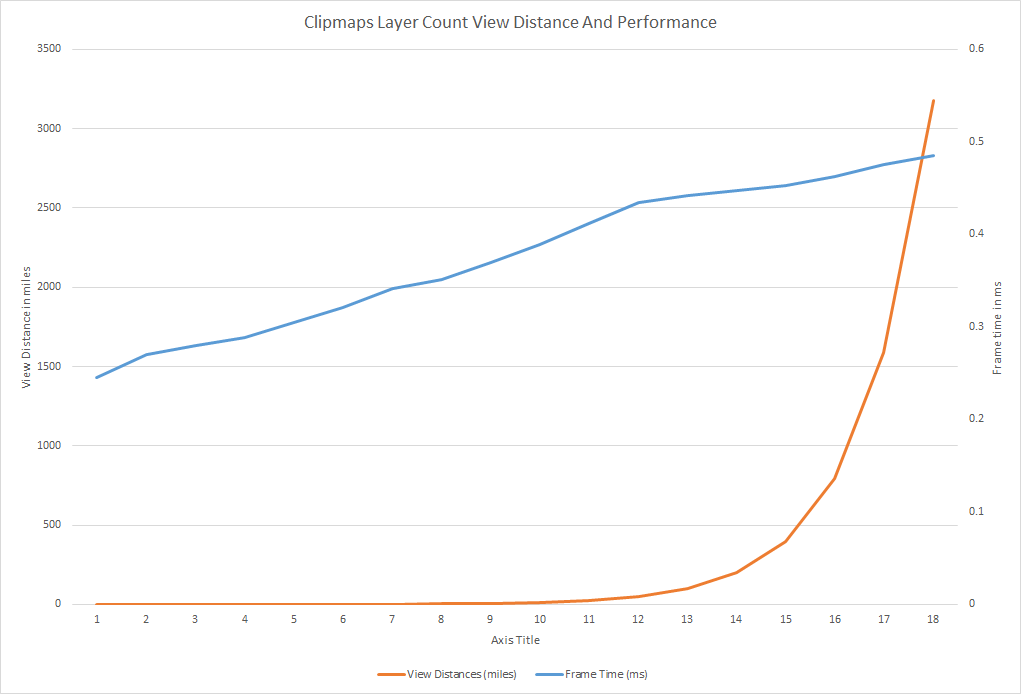
\includegraphics[width=1.0\textwidth]{figures/clipmaps_plot_1.png}
	\caption{
		View distance and render time for a given number of clipmap layers.
	}
	\label{fig:clipmaps_plot_1}
\end{figure}

There is a linear relationship between frame time and layer count, but an exponential relationship between view distance and layer count.
For a relatively minor increase in frame time an absurd view distance of over 3000 miles can be achieved.
For reference, the largest possible view distance on earth is around 300 miles, between two mountains in South America. \cite{viewdistancemaxearth}

Larger individual layer sizes increase view distance and reduce polygon screen-space at the cost of performance.
\editor{Graph of performance over size of layers}

The addition of a geometry shader normal calculation simplifies the terrain generation process and improves visual quality, but incurs a small performance hit.
\editor{Geometry shader normal calculation performance hit}


\section{Vegetation}

The far layers of the vegetation system are rough visual approximations of the closeup tree meshes, but are significantly less costly for rendering.
\editor{Graph of performance meshes vs. impostors vs. batched simple geometry}

Increasing the size of tree groups decreases CPU performance while improving rendering performance.
\editor{Graph of chunk size performance}


\section{Water}


\section{Depth Buffer Precision}

Our system supports very large view distances.
Setting the far plane at sufficient distance for our scene significantly degrades the performance of the depth buffer, even with 32 bits of precision.

The problem is that the depth buffer stores reciprocal depths, such that most of the depth buffer is alloted for nearby fragments.
To improve depth buffer performance for far distances, we use the inverted depth buffer trick.
By using a DirectX compatibility feature of OpenGL, we can use a depth buffer ranging from zero to one instead of negative one to one.
Then, by storing depths reversed from the conventional direction, we can utilize the inherent distribution of floating point precision to even out the distribution of depth values in our scene.
The conventional depth direction has near values at zero and far values at one.
However, floating point precision is higher for values closer to zero.
By storing near depths at one and far depths at zero, the additional floating point precision creates a pseudo-logarithmic distribution of depth values.

This results in a significant reduction in depth fighting artifacts.
See figure \editor{comparison of reverse depth turned off and on}.



\iffalse \bibliography{../bibliography.bib} \fi

\chapter{Future Work}

\section{Terrain Lighting}

\subsection{Shadows}

Besides the HBAO+ post-processing pass applied to the whole scene, no shadows are currently calculated.
The scene is inherently difficult to shadow due to the large view scales.
A cascaded shadow map system with robust view frustum culling could be applied to the geometry clipmap layers but the performance hit on rendering may be significant.

One option to improve rendering performance is horizon-based shadowing.
Horizon-base shadowing pre-calculates horizon values for each pixel in a heightmap.
These horizon values are then compared against sun elevation to determine whether a fragment is in shadow.

While calculating horizon values for all clipmap layers may be expensive, it might be possible to calculate horizon values for e.g. every fourth layer and re-use the low resolution horizontal values in high resolution layers.


\subsection{Accurate Scattering}

Our current scattering system is a very rough approximation of real scattering.
There are open source solutions with more accurate simulations of the Rayleigh and Mie scattering which could be used.

It might also be better to use a non-photo-realistic color-ramp scattering simulation such as the one used by Firewatch.


\subsection{Volumetric Lighting}

Nvidia Gameworks, which our system uses for screen-space ambient occlusion, also has an implementation of volumetric lighting that could be used for more accurate sunset and sunrise effects.


\section{Water}

Our water system uses the shape of geometry clipmaps for simplicity but this causes a lot of water vertices to be rendered off-screen.
Using a grid projected from screen-space is a common way to render water at different view scales.


\section{Terrain Generation}

Our system uses a standard grid to store the world map, but this brings some square artifacts into the large-scale terrain features.
Other similar systems use a Voronoi diagram to produce more varied large-scale structure.


\section{Vegetation}

While the mesh facade rendering system is cheap, it is a very rough visual approximation of distance forests.
It is also not sufficiently cheap to render at significant scale.
As such, the current system has a much shorter view distance for vegetation than it does for terrain.

Using a GPU ray-cast simulation of forests could produce much larger view distances and improved visual approximation. \cite{terraintreecast}



\nocite{*}
\bibliography{bibliography}

% Indents Appendix in Table of Contents
\makeatletter
\addtocontents{toc}{\let\protect\l@chapter\protect\l@section}
\makeatother

% Hack to make Appendices to appear in Table of Contents
\addtocontents{toc}{%
   \noindent APPENDICES
}
\begin{appendices}


\end{appendices}

\end{document}
